\section{Was erkannt werden soll}
\name{mec-2} modelliert Mechanismen durch
sogenannte \name{Nodes} und \name{Constraints}.
Die Gelenke sind entsprechend als Nodes und Glieder als Constraints zu betrachten.
Beispielhaft für ein Viergelenk sähe das generierte JSON gemäß Abbildung \ref{fig:4bar} aus.

\begin{figure}
  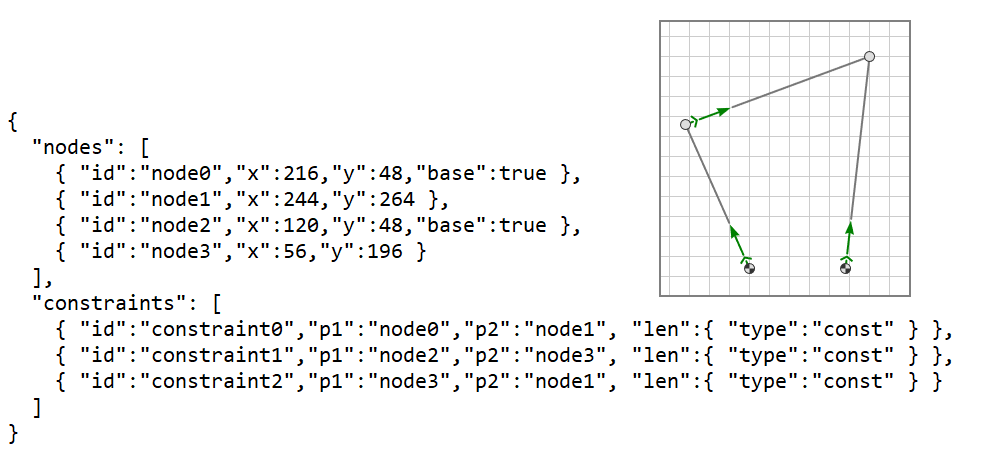
\includegraphics[width=\textwidth]{images/4bar_json}
  \caption{Die JSON-Darstellung eines durch mec-2 erstellten Viergelenks mit dem entsprechend generierten Mechanismus.}
  \label{fig:4bar}
\end{figure}

Um diesen Mechanismus durch eine Handzeichnung zu erstellen, ist es erforderlich, einen Algorithmus zu trainieren, der in der Lage ist, mit einer entsprechenden Skizze als Input solchen JSON-Code als Output zu produzieren.

Hierfür mussten zunächst Trainingsdaten geschaffen werden, anhand derer ein solcher Algorithmus Merkmale erlernen kann, die eine Zuordnung der Eingangsbilder zu den entsprechenden Lösungen bilden kann.
Es wurden etwa 1200 Nodes, 1200 Base-Nodes und 1200 nicht zutreffende Bilder erstellt, welche vor dem Training durch Rotation und Spiegelung augmentiert wurden, um die Varianz der Trainingsdaten zu erhöhen.

Des weiteren, wurden von \name{mec-2} genutzte Symbole dem Trainingsset hinzugefügt, sodass der Algorithmus diese nicht als Nodes erkennt, damit Mechanismen erweitert werden können, ohne die bereits erkannten Elemente nochmal zu erkennen.

\begin{figure}
  \centering
    \begin{subfigure}[b]{0.4\textwidth}
        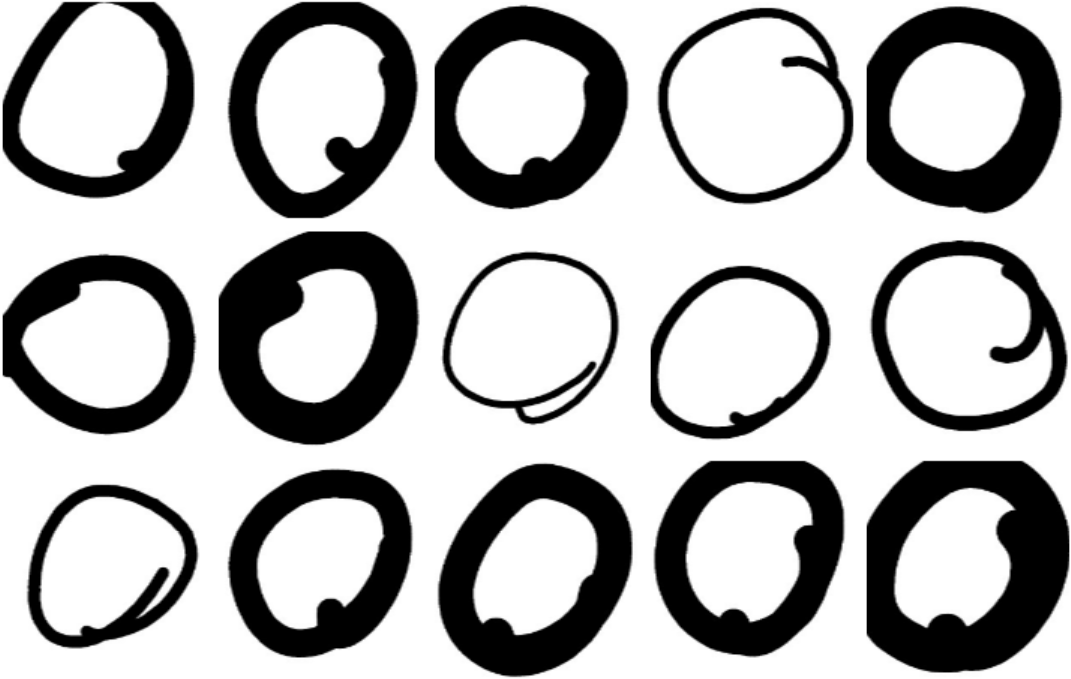
\includegraphics[width=\textwidth]{images/os.png}
        \caption{lose Nodes}
        \label{fig:os}
    \end{subfigure}
    \begin{subfigure}[b]{0.4\textwidth}
        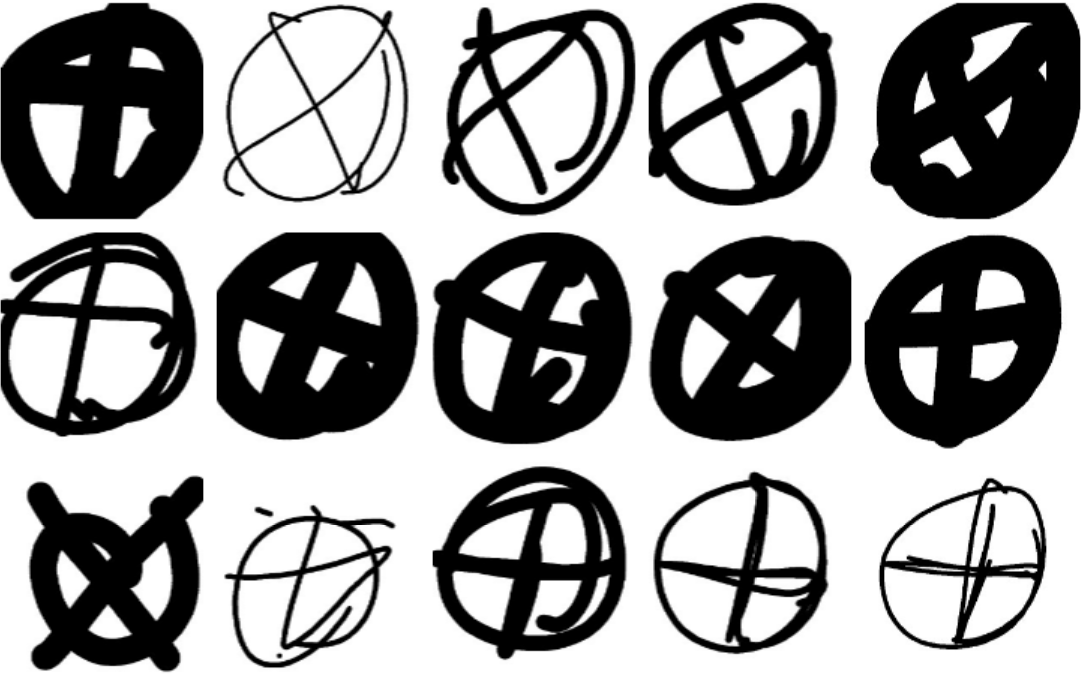
\includegraphics[width=\textwidth]{images/xs.png}
        \caption{Base-Nodes}
        \label{fig:xs}
    \end{subfigure}
    \begin{subfigure}[b]{0.4\textwidth}
      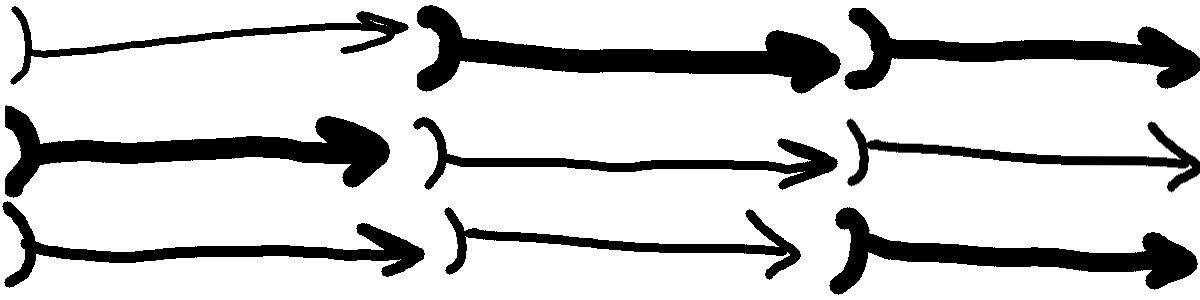
\includegraphics[width=\textwidth]{images/rs.png}
      \caption{rotatorische Constraints}
      \label{fig:rs}
    \end{subfigure}
    \begin{subfigure}[b]{0.4\textwidth}
      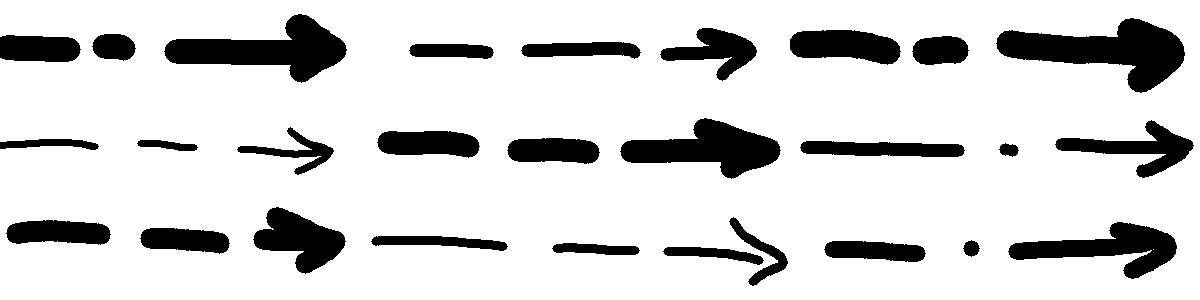
\includegraphics[width=\textwidth]{images/ts.png}
      \caption{translatorische Constraints}
      \label{fig:ts}
    \end{subfigure}
    \caption{Beispiele für handgezeichnete Symbole welche zum Trainieren der Algorithmen genutzt werden.}
    \label{fig:example_symbols}
\end{figure}

Neben den Nodes wurden für die Constraints wieder 1200 rotatorische und 1200 translatorische Verbindungen gezeichnet, welche sich in ihrer Gestaltung an die Darstellung von Constraints an Abbildung \ref{fig:constraints_gtk} orientieren.
Für gebundene und freie Constraints gibt es noch keine Trainingsdaten, da diese für die momentan bestimmte Funktion zunächst irrelevant sind.

\begin{figure}
  \centering
  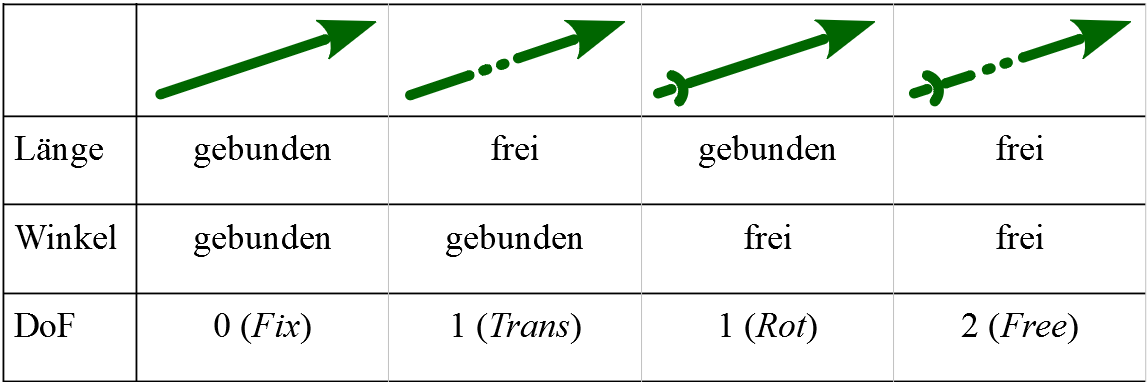
\includegraphics[width=0.8\textwidth]{images/gtk2019_tab1.png}
  \caption{Darstellung der Constraints in ihren unterschiedlichen Auslagemöglichkeiten. Auszug von Tabelle 1 des Beitrags von Prof. Gössner zum Sammelband des Getriebetechnischen Kolloquiums 2019 in Dortmund\cite{Goessner2019a}}.
  \label{fig:constraints_gtk}
\end{figure}
